  \mysection{The Sellsword}{trope-sellsword}

  \flavor{
    How heavy this axe \\
    Burden carried from birth \\
    Wrought in Stygian visions \\
    By the gods of the earth \\
    \Tilde The Sword, "How Heavy this Axe"
  }

\begin{center}
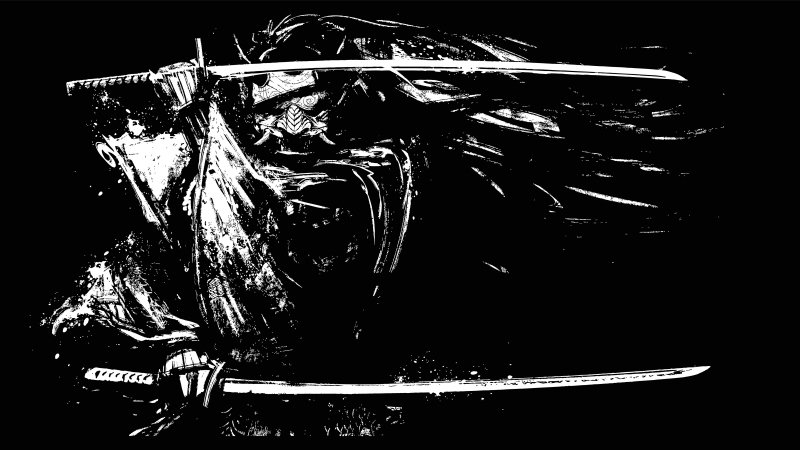
\includegraphics[width=\linewidth,keepaspectratio=true]{tropes/SellswordHeader}
\end{center}


  \mysubsection{Creation}{sellsword-creation}

  Write down the following information on your \mylink{Adventurer Sheet}{adventurer-sheet.6}
  
  \callout {
    \mynumlist {
        \item You start with \mybold{6 Flesh and 6 Grit}.
        \item Move your \VIG \DCUP (to a d10). Pick \DEX, \INT, or \FOC and move it \DCDOWN (to a d6).
        \item If you need to \RSTRY{\VIG}, you only fail on a natural 1 (instead of a 1 or 2). Put a check next to \VIG on your Adventurer Sheet so you don't forget.
        \item You have d4 \mylink{Prowess}{sellsword-prowess} that you can use in \mylink{Combat}{combat}.
        \item Choose three different \mylink{Virtues}{sellsword-virtues} and a \mylink{Complication}{sellsword-complications}. Modify your sheet as necessary.
        \item Write down your \mylink{Starting Gear}{sellsword-starting-gear}.
    }
 }

\newpage
\begin{multicols*}{2}\raggedcolumns


  \mysubsection{Prowess}{sellsword-prowess}

  Your Prowess is a Resource Die whose result can be added to \mybold{any} \mylink{Combat Action}{combat-combat-actions} or \mylink{Guarding Action}{combat-guarding} try. If you apply the result of a Prowess try to a Combat Action, you also add the result to your damage (this damage is applied \mybold{after} \mylink{Lethal damage}{combat-damage-lethal}, if applicable). You can roll your Prowess \myital{after} your try is rolled (it doesn't have to be at the same time), but you can only roll it once per Moment. 

Your Prowess starts at \UDD{d4}, and moves \DCDOWN on a Failure.




  \myhighlight{Mortal}{sellsword-mortal}
    
  You are creature of Order, and possess a soul - and are thus \mybold{Hallowed}.


  \myimage{tropes/Sellsword_1}

\cbreak

\mysubsection{Starting Sellsword Virtues}{sellsword-virtues}

    \begin{center}
        \myredbold{\large{Choose 3 of the following}}
    \end{center}


    \myhighlight{Blademaster}{sellsword-virtue-blademaster}

    \callout {
    \mynumlist {
        \item Two-Handed weapons only count as one \mylink{Burden}{gear-burden} instead of two
        \item You can wield any \DEX weapon as if it were a \VIG weapon (see \mylink{Gear: Weapons}{gear-weapons} for more info)
    }}


    \myhighlight{Charms}{sellsword-virtue-vulgate-charms}

    You can perform the \mylink{Vulgate of Charms}{vulgate-charms} at will.


    \myhighlight{Deadly}{sellsword-virtue-deadly}

    You deal \mylink{Lethal damage}{combat-damage-lethal} with any \VIG weapon you wield (see the section on \mylink{Damage}{combat-dealing-damage} under \mylink{Combat}{combat} for more info).


    \myhighlight{Harder Than a Coffin Nail}{sellsword-virtue-coffin-nail}

    \flavor{It turned out that the sweet-talking, tattoo-sporting pikey was a gypsy bare-knuckle boxing champion. \Tilde "Snatch"}

    \mybullet {
        \item Your \INJURY starts at \mybold{Solid (d4)};
        \item You deal +1 damage dealing \mylink{Unarmed}{combat-damage-unarmed} damage; and
        \item You gain +2 Flesh.
    }
    \myhighlight{Medicine}{sellsword-virtue-vulgate-medicine}

    You can perform the \mylink{Vulgate of Medicine}{vulgate-medicine} during the \mylink{Shopping Step}{downtime-shopping} of \mylink{Downtime}{downtime}.

\newpage

    \myhighlight{Hunter}{sellsword-virtue-hunter}

    You start the game with:

    \callout {
      \mybullet {
        \item a suit of \mylink{Light Armor}{gear-armor};
        \item a \mylink{Strongbow}{gear-vig-weapons};
        \item a \mylink{Quiver of Arrows}{gear-equipment};
        \item a \mylink{Spear}{gear-vig-weapons}
      }
    }




    \myhighlight{My Father's Sword}{sellsword-virtue-fathers-sword}

    You start the game with any \mylink{\VIG Weapon}{gear-vig-weapons} of your choice. \mybold{With this \myital{specific} weapon (only)}:
    \callout {
    \mynumlist {
        \item Your Attack \RO is +4;
        \item You deal \mylink{Lethal damage}{combat-damage-lethal}; and
        \item You cannot be \mylink{Disarmed}{effect-disarmed}
    }}

    If you lose this weapon, you lose the abilities that go with it. Describe to the Arbiter what makes this weapon unique.


    \myhighlight{Sacraments}{sellsword-virtue-vulgate-sacraments}
   
    You gain a single Grace die (d4) which allows you to perform the \mylink{Vulgate of Sacraments}{vulgate-sacraments}.


    \myhighlight{Second Skin}{sellsword-virtue-second-skin}
    \callout {
    \mynumlist {
        \item Your Armor doesn't count toward your \mylink{Burden}{gear-burden};
        \item You can repair 1 \UD of your Armor when you take a \mylink{Breather}{combat-resting-breather}, up to its \MAX \UD;
        \item You start the game with a suit of \mylink{Medium Armor}{gear-armor} or \mylink{Heavy Armor}{gear-armor}
    }}

    This Armor looks very unique. Describe what it looks like to the Arbiter.

\cbreak

    \myhighlight{Three Kills Per Stroke}{sellsword-virtue-three-kills}

    If you strike a killing blow against a Monster, you may immediately take another \mylink{Attack Action}{combat-attack-action} against a Close Monster. You may continue in this way as long as you deliver a killing blow to a Monster. See the section on \mylink{Combat}{combat} for more information on Combat Actions.

    \myhighlight{Veteran}{sellsword-virtue-veteran}

    This isn't your first rodeo - you have some experience with a prior \mylink{Band}{roles-band}. You start with +4 Grit. Tell the Arbiter the name of your old Band, and what happened to them.


    \myhighlight{Why Won't You Stay Down?!}{sellsword-virtue-stay-down}


    \callout {
        \mynumlist {
    
        \item Choose one \mylink{Save}{adventurer-saves} (including the one you chose at character creation) and raise it one rank i.e. from Defenseless(d4,+0) to Preserved(d8,+1) or Preserved(d8,+1) to Protected(d12,+2);
        \item Your \DEATH starts at \mybold{Tough (d4)}; and
        \item Once per Session, just before you are about to roll a \Duration for your Adventurer, you may instead choose to immediately end the effect.
        }
    }



    \mysubsection{Sellsword Complications}{sellsword-complications}

    \begin{center}
        \myredbold{\large{Choose 1 of the following}}
    \end{center}


    \myhighlight{Alcoholic}{sellsword-complication-alcoholic}

    You are addicted to \mylink{Alcohol}{gear-narcotics-alcohol}. Whenever you take a \mylink{Breather}{combat-resting-breather}, you have to take at least one drink or you heal no Grit; whenever you take a \mylink{Bivouac}{combat-resting-bivouac}, you must take at least one drink or gain none of the beneficial effects of resting. \RSTRY{\VIG} at the end of the Bivouac - if you fail, you are \mylink{Hung Over}{effect-hung-over}.

\newpage

    \myhighlight{Cheap Tricks}{sellsword-complication-cheap-tricks}

    You do not like or trust magic or the unnatural. Your dislike extends to \mylink{Philosophers}{trope-philosopher} and \mylink{The Unseelie}{the-inhabitants}. The degree to which you feel this way is up to you. Let the Arbiter know why.

    \myhighlight{The Cimmerian}{sellsword-complication-cimmerian}

    Your appearance is so outlandish, barbaric, out-sized, etc. that even educated and well-traveled people will stop to stare at you. People can pick you easily out of a crowd, and your reputation precedes you.

    \myhighlight{Credo}{sellsword-complication-credo}
  
    You must make a vow - a short, specific, personal statement that you will not forget. For example, "I will protect my friend Johann" or "I will never harm an unarmed person". You must follow this vow to the best of your ability.

    \myhighlight{Filthy}{sellsword-complication-filthy}

    You refuse to bathe except under the most dire circumstances. Your general hygiene is horrible. If you're using \mylink{Persuasion}{arbiter-persuasion}, you can never seduce someone (intimidate is a different story), and if you're downwind from \mylink{Monsters}{monsters} it might affect your ability to get the Drop on them.

    \myhighlight{Hippophobia}{sellsword-complication-hippophobia}

    You are afraid of horses and mules. You refuse to ride one (riding in a cart is OK).


    \myhighlight{Honorable}{sellsword-complication-honorable}

    You refuse payment for good deeds, always rescue the helpless, and refuse to fight unarmed foes (within reason, of course). 

    \myhighlight{Mortal Enemy}{sellsword-complication-mortal-enemy}

    You have a mortal enemy, someone powerful who has done you significant wrong. This enemy should be substantially more powerful than you. You are driven by your revenge against this mortal enemy. Tell the Arbiter who they are, and why they are your enemy.

    \myhighlight{Pit Fighter}{sellsword-complication-pit-fighter}

    You strongly believe that combat should take place between two people face-to-face. You won't use Shoot weapons, and you'll never throw a Throw weapon at a target.

    \myhighlight{Sins of the Father}{sellsword-complication-sins-father}

    Your parent (alive or dead) is infamous. If people ever discover that you are their child, they will have significant negative reactions. At the Arbiter's complete discretion you will encounter various assassins, sellswords, and kidnappers who have figured out who you are, and want to do you harm. Tell the Arbiter a bit about this parent.

 
  \mysubsection{Sellsword Starting Gear}{sellsword-starting-gear}

    In addition to any gear you might have gained from Virtues, you have:

\callout{\footnotesize{
  \mybullet {
    \item 6 iron pieces; 
    \item a worn bedroll;
    \item a backpack;
    \item \UDD{d4} of \mylink{Personal Provisions}{gear-equipment};
    \item one pitted \mylink{Shield}{gear-armor} OR one rusty \mylink{Helmet}{gear-armor} OR one \mylink{Spear}{gear-vig-weapons};
    \item one pick OR 3 rolls on the \mylink{Random Items}{appendix-a-random-items} table in Appendix A
  }}}


    \myhighlight{What Next?}{sellsword-what-next}

    The Sellsword is built for \mylink{Combat}{combat}; the section on \mylink{Fighting}{combat-fighting}, including \mylink{Maneuver Actions}{combat-maneuvers}, and \mylink{Combat Actions}{combat-combat-actions} should be the next thing you check out.



\end{multicols*}

